% =========================================================================
% Stage 6.5 section: variance-based global sensitivity analysis (GSA) of
% the Phase 1 engine. Drop-in for the methodology-results seam of the
% thesis (written as a chapter section, like the Japanese validation
% section; the machine-readable records live in the repository under
% docs/decisions/adr0033-gsa-study-*.json and the method decisions in
% ADR-0033).
%
% New BibLaTeX keys (entries PROVIDED in _thesis_gsa.bib; merge into the
% thesis .bib or \addbibresource that file):
%   saltelli_primer_2008, saltelli_2002, saltelli_2010, jansen_1999,
%   sobol_1993, homma_saltelli_1996, mara_tarantola_2012, kucherenko_2012,
%   owen_1997, archer_1997, schweckendiek_2014
% Existing keys reused: sellmeijer_2011, pol_sie_2024, pol_compgeo_2024
% Figures: figures/gsa_indices_kp58_8_matrix.png,
%   figures/gsa_levels_kp58_8_matrix.png,
%   figures/gsa_interaction_kp58_8_matrix.png,
%   figures/gsa_convergence_kp58_8_matrix.png, figures/gsa_companions.png
%   (canonical copies regenerate from scripts/gsa_study.py into
%   docs/figures/).
% =========================================================================

\section{Global Sensitivity Analysis of the Phase 1 Engine}
\label{sec: Global Sensitivity Analysis}

The Phase~1 engine maps an eight-dimensional stochastic input space, the
seven-parameter vector $\theta$ of Section~\ref{sec: Overview of the
Three-Phase Computational Architecture} plus the stochastic seepage length
$L$, onto the static and transient fragility deliverables. The fragility
curves themselves do not reveal \emph{which} inputs drive the failure
probabilities, how much of the static-transient bias each parameter carries,
or how strongly the multiplicative $C_e \times k_{aq}$ progression-rate
interaction contributes beyond its separate main effects. This section
quantifies exactly that with a variance-based global sensitivity analysis in
the framework of \textcite{saltelli_primer_2008}: first-order Sobol' indices
$S_i$ for the factor prioritization setting (which input, if it could be
fixed, would reduce the output variance most) and total-effect indices
$S_{Ti}$ for the factor fixing setting (which inputs are noninfluential and
could be frozen), with the gap $S_{Ti} - S_i$ as the model-free measure of
each input's involvement in interactions. Every methodological decision
below is recorded as ADR-0033 in the repository decision log; the analysis
wraps the engine unchanged and consumes it through the same vectorized
evaluator as the production sweep.

\subsection{Method}
\label{subsec: GSA Method}

\paragraph{Variance decomposition.}
For a square-integrable model output $Y = f(X_1, \ldots, X_k)$ with mutually
independent inputs, the variance admits the unique orthogonal
(ANOVA-HDMR) decomposition
$V(Y) = \sum_i V_i + \sum_{i<j} V_{ij} + \ldots$
\parencite{sobol_1993, saltelli_primer_2008}, from which
\begin{equation}
  S_i \;=\; \frac{V\!\left[\,\mathbb{E}(Y \mid X_i)\,\right]}{V(Y)},
  \qquad
  S_{Ti} \;=\; \frac{\mathbb{E}\!\left[\,V(Y \mid X_{\sim i})\,\right]}{V(Y)}
  \;=\; 1 - \frac{V\!\left[\,\mathbb{E}(Y \mid X_{\sim i})\,\right]}{V(Y)},
  \label{eq:sobol-definitions}
\end{equation}
where $X_{\sim i}$ denotes all inputs but $X_i$. $S_i$ is the main-effect
share of the output variance; $S_{Ti}$ adds every interaction term involving
$X_i$, so $S_{Ti} \geq S_i$ always, $\sum_i S_i = 1$ characterizes an
additive model, and $S_{Ti} \approx 0$ is necessary and sufficient for
$X_i$ to be noninfluential \parencite{homma_saltelli_1996,
saltelli_primer_2008}.

\paragraph{Quantities of interest.}
Sobol' analysis requires a scalar output per input draw. Four are analyzed,
all computed from one engine pass per conditioning level $h_i$ so the
shared-sample contract extends to the sensitivity analysis itself:
the transient failure indicator $Y_1 = \mathbf{1}\{Z_{\mathrm{trans}} \leq
0\}$ (the primary reliability QoI; for a binary output $V(Y) = P_f(1 -
P_f)$, so the indices decompose the variance of the fragility deliverable
directly); the static failure indicator $Y_2 = \mathbf{1}\{Z_{\mathrm{stat}}
\leq 0\}$ (the comparator; because $Y_1$ and $Y_2$ are evaluated on the same
sample, differences between their index vectors attribute the
static-transient bias to specific inputs); the final erosion fraction
$Y_3 = \ell_{e,\mathrm{final}}/L$ (a continuous progression measure that
retains information below the failure threshold); and the static margin
$Y_4 = Z_{\mathrm{stat}} = H_c - (h_i - z_{\mathrm{toe}})$ (the pure
Sellmeijer resistance sensitivity; since the level enters only as an
additive constant, its decomposition is level-invariant). Two candidate
QoIs were rejected with recorded rationale: the median time to breach is
defined only on the breached subset (about a quarter of the draws at the
design level), and conditioning the output on the output breaks the
unconditional decomposition underlying
Equation~\eqref{eq:sobol-definitions}; a per-draw bias factor
$Z_{\mathrm{stat}}/Z_{\mathrm{trans}}$ mixes incommensurable margins and
degenerates at zero crossings, the bias being a population functional of the
two curves rather than a per-realization random variable.

\paragraph{Input space and the correlation question.}
The analyzed input space is the production prior itself: the seven $\theta$
marginals of the section configuration (including the $d_{70}$ physical
bounds) plus the lognormal seepage length $L$ (mean equal to the geometric
$L$, coefficient of variation 0.20), giving $k = 8$. Standard Sobol'
indices presuppose independent inputs; the k$_{aq}$-d$_{70}$ coupling
question was resolved empirically in ADR-0012 as the two-population
decoupling (the erodible sand matrix and the water-bearing gravel framework
are distinct soils, sampled from their own marginals with no imposed
correlation), so under the production prior all eight inputs are mutually
independent and the decomposition in
Equation~\eqref{eq:sobol-definitions} holds exactly, with no
approximation to bound. The consequence of a hypothetical residual
dependence is nevertheless quantified rather than dismissed: a bounding
companion run imposes the retired provisional Gaussian-copula correlation
$\rho_{\ln} = 0.6$ between $k_{aq}$ and $d_{70}$ (about six times the
pooled empirical estimate) and performs the analysis in the space of the
independent copula generators, i.e.\ through the Rosenblatt transform, in
both conditioning orders. In that construction the anchored variable's
index is its full contribution including the correlated share and the other
pair member's index is its independent (decorrelated) contribution,
recovering the dependent-input indices of \textcite{mara_tarantola_2012}
and \textcite{kucherenko_2012} exactly for a Gaussian copula while reusing
the independent-input estimator stack unchanged. Naively applying
independent-input formulas to correlated physical samples, which silently
invalidates the decomposition \parencite[p.~162]{saltelli_primer_2008}, is
thereby avoided.

\paragraph{Design, estimators, and computational budget.}
The sample design is the two-matrix scheme of \textcite{saltelli_2002}, as
presented in \textcite[\S 4.6]{saltelli_primer_2008}, in its radial form:
base matrices $A$ and $B$ and the $k$ spliced matrices $A_B^{(i)}$ ($A$
with column $i$ from $B$), at a cost of $N(k+2) = 10N$ engine evaluations
per replicate. The matrices are drawn from an Owen-scrambled Sobol'
low-discrepancy sequence in $2k$ dimensions \parencite{owen_1997}, the
Primer's own recommendation for these designs. The estimators are the
current best practice of \textcite{saltelli_2010}, superseding the original
formulations printed in the Primer, a deliberate and recorded extension:
\begin{equation}
  \widehat{S}_i = \frac{\frac{1}{N}\sum_{j=1}^{N}
      y_B^{(j)}\left(y_{A_B^{(i)}}^{(j)} - y_A^{(j)}\right)}{\widehat{V}},
  \qquad
  \widehat{S}_{Ti} = \frac{\frac{1}{2N}\sum_{j=1}^{N}
      \left(y_A^{(j)} - y_{A_B^{(i)}}^{(j)}\right)^2}{\widehat{V}},
  \label{eq:estimators}
\end{equation}
the total-effect form being Jansen's \parencite{jansen_1999}, whose
numerator is non-negative by construction. The base sample is $N = 2^{13} =
8192$ with $R = 25$ independent scramblings per conditioning level (about
$2 \times 10^6$ engine realizations per level), a budget justified by the
convergence ladder below rather than asserted; the accelerated engine
(ADR-0029/0030) evaluates one replicate design in roughly a tenth of a
second, so the full two-section study completes in minutes.

\paragraph{Uncertainty and convergence.}
Every reported index carries two independently constructed 95\,\%
confidence intervals. The primary interval is the Student-t interval over
the $R = 25$ independent scramblings, the unbiased randomized
quasi-Monte-Carlo error statement; the cross-check is the row bootstrap of
the paired design outputs recommended by the Primer
\parencite[p.~166]{saltelli_primer_2008, archer_1997}, with $B = 500$
resamples, pooled across replicates at the level of the replicate-mean
index. Agreement between the two interval families is itself a
health check and held throughout (the widest discrepancies remain within
about a percent of index value). Convergence is demonstrated with an
$N$-ladder $N \in \{2^{10}, 2^{11}, 2^{12}, 2^{13}\}$ at fixed $R$; the
pre-registered acceptance criterion (ADR-0033) is an absolute index drift
below 0.02 between the two finest rungs for every reported index, plus the
structural invariants $S_{Ti} \geq S_i$, $\sum_i S_i \leq 1$ within noise,
and exact zeros where the architecture guarantees them.

\paragraph{Validation of the machinery.}
Before touching the engine, the estimator stack was validated against four
analytical benchmarks with known indices, mirroring the Primer's own test
cases: the Ishigami function (interactions and a pure-interaction factor;
agreement within 0.01 absolute), the Sobol' g-function at $k = 8$ (the
engine's dimensionality; within 0.015), a linear-Gaussian threshold
indicator with quadrature ground truth (the binary-QoI case the engine
analysis leans on; within 0.02), and a correlated lognormal pair pushed
through the production copula construction with closed-form full and
independent indices (validating the Rosenblatt companion; within 0.015).
Two bit-identity guards pin the analysis to the production engine: the
generator-to-physical input map reproduces the M2 sampler exactly, and the
continuous-output evaluator adapter reproduces the failure flags of the
production batch evaluator exactly. Consistently, the design-level failure
probabilities recovered by the GSA sample match the $N = 10^5$ production
sweep values to three decimals (for example transient $P_f = 0.263$ against
the sweep's $0.263$ at KP58.8, $h = 41.0$\,m).

\paragraph{Scenario axis.}
Per the shape-invariance finding of the climate-axis analysis (ADR-0023),
one canonical d4PDF event shape drives the conditioning sweep for all
scenarios, so a separate +4K sensitivity analysis at matched conditioning
level would be evaluating the identical deterministic loading record; the
driver verifies this bit-identity and records it in the study metadata
rather than spending a redundant sweep. The climate-relevant sensitivity
statement is instead the \emph{level dependence} of the indices reported
below: warming shifts the peak-stage distribution upward along the
conditioning axis, so the rotation of the index picture from shoulder to
upper levels is precisely how the parameter importance picture shifts under
+4K.

\subsection{Results}
\label{subsec: GSA Results}

The analysis covers the two governing cross-sections in which backward
erosion is genuinely reachable at attainable stages, KP58.8 and KP60.0
(matrix $d_{70}$ interpretation), at four conditioning levels each,
spanning the fragility shoulder, the design high water level, the
transition, and the upper bulk. Figure~\ref{fig:gsa_indices} presents the
design-level indices for all four QoIs at KP58.8;
Table~\ref{tab:gsa_design_indices} tabulates the transient-indicator
indices for both sections.

% --- Figure 1: design-level indices, KP58.8 ---
\begin{figure}[htbp]
  \centering
  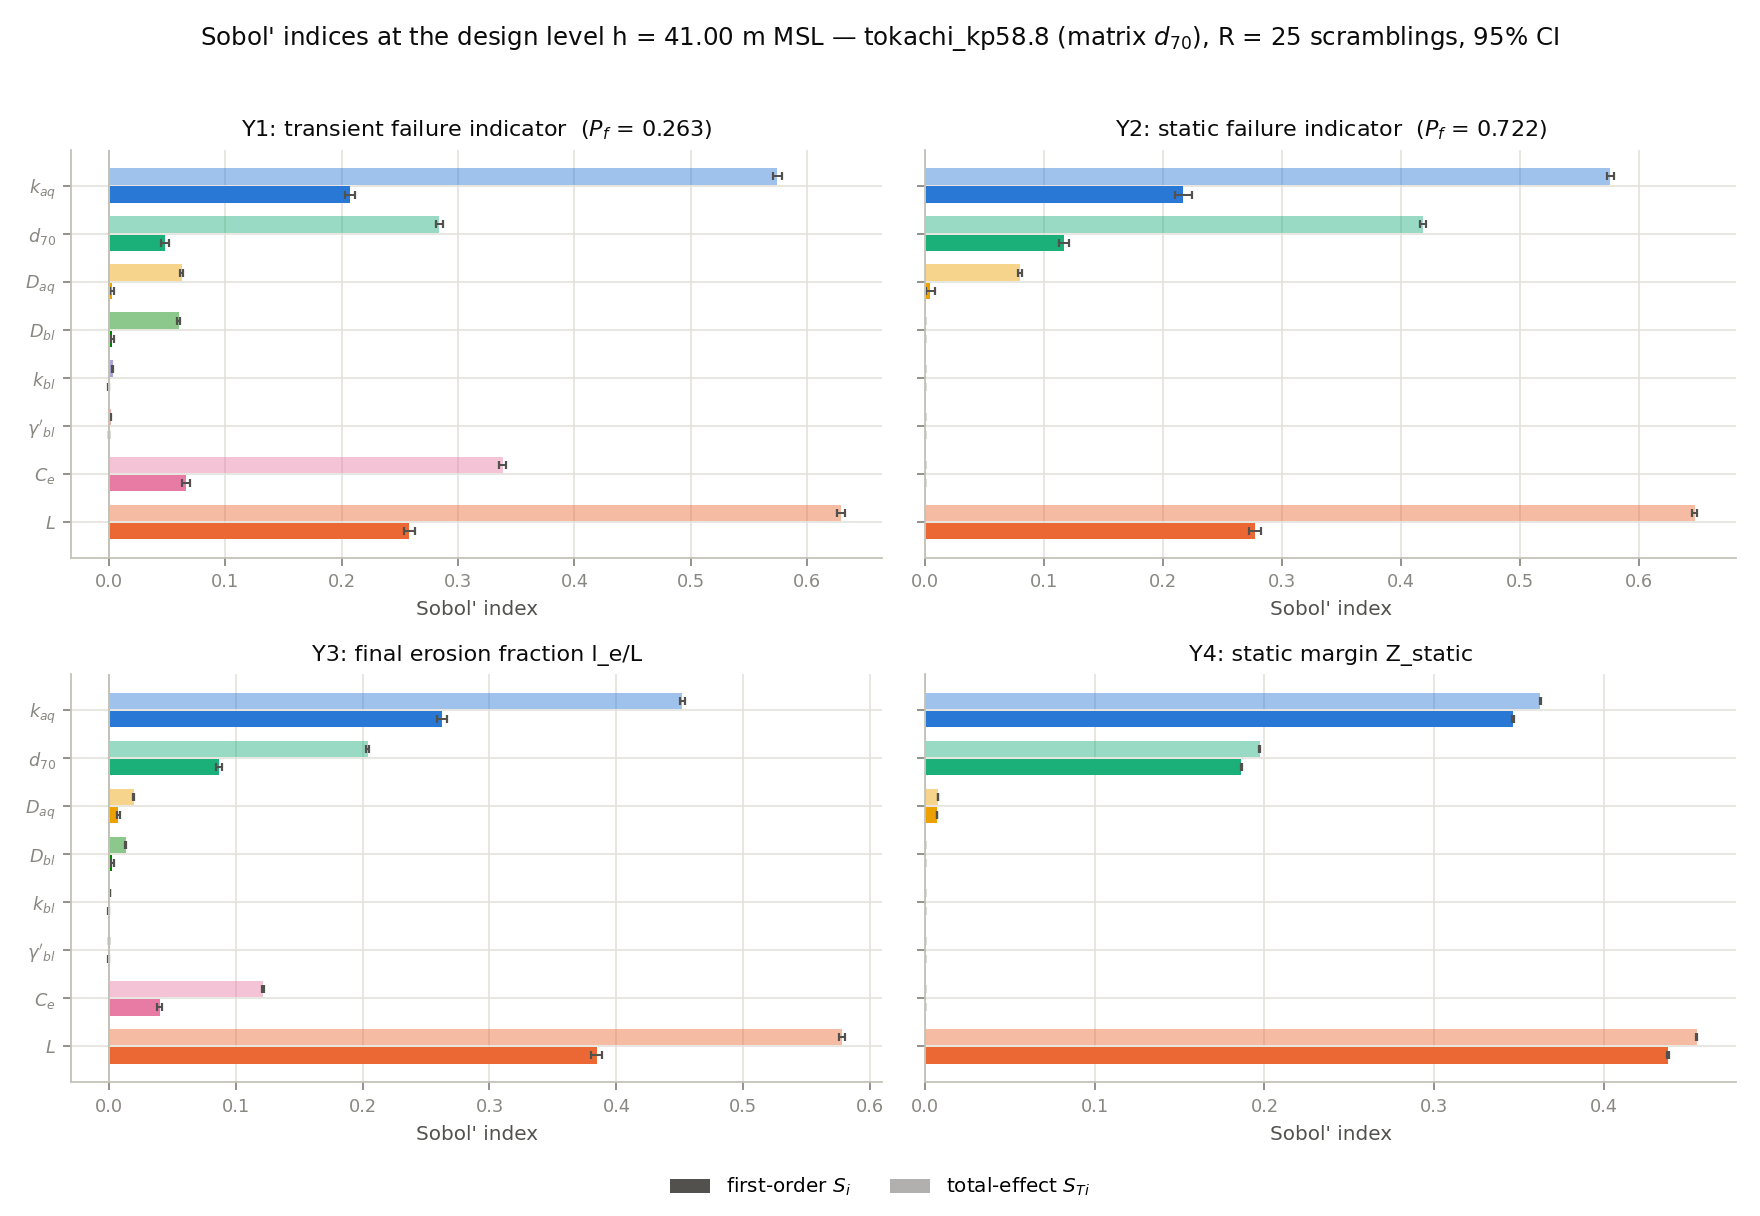
\includegraphics[width=\textwidth]{figures/gsa_indices_kp58_8_matrix.png}
  \caption[Sobol' indices at the design level, KP58.8]{First-order
    ($S_i$, solid) and total-effect ($S_{Ti}$, translucent) Sobol' indices
    with 95\,\% replicate confidence intervals for the four QoIs at the
    design level $h = 41.0$\,m MSL, KP58.8 (matrix $d_{70}$), $R = 25$
    scramblings of $N = 8192$. The static QoIs (right column) carry exact
    structural zeros for $C_e$, $D_{bl}$, $k_{bl}$, and $\gamma'_{bl}$, as
    the architecture requires; the transient indicator (top left) shows
    the large total-effect-minus-first-order interaction gaps on $L$,
    $k_{aq}$, $C_e$, and $d_{70}$.}
  \label{fig:gsa_indices}
\end{figure}

% --- Table: transient-indicator indices at the design levels ---
\begin{table}[htbp]
  \centering
  \caption[Sobol' indices of the transient failure indicator at the design
    levels]{First-order and total-effect Sobol' indices of the transient
    failure indicator $Y_1$ at the design levels of the two governing
    cross-sections (matrix $d_{70}$; $N = 8192$, $R = 25$ scramblings;
    $\pm$ half-widths of the 95\,\% replicate confidence intervals; the
    pooled bootstrap intervals agree within about 0.005 throughout).
    Small negative first-order estimates for noninfluential inputs are the
    expected estimator behavior near zero
    \parencite[p.~170]{saltelli_primer_2008}.}
  \label{tab:gsa_design_indices}
  \begin{tabular}{l rr rr}
    \toprule
    & \multicolumn{2}{c}{KP58.8, $h = 41.00$\,m ($P_f = 0.263$)}
    & \multicolumn{2}{c}{KP60.0, $h = 42.75$\,m ($P_f = 0.314$)} \\
    \cmidrule(lr){2-3} \cmidrule(lr){4-5}
    Input & $S_i$ & $S_{Ti}$ & $S_i$ & $S_{Ti}$ \\
    \midrule
    $k_{aq}$        & $0.207 \pm 0.004$ & $0.574 \pm 0.004$
                    & $0.252 \pm 0.004$ & $0.606 \pm 0.003$ \\
    $d_{70}$        & $0.048 \pm 0.003$ & $0.284 \pm 0.003$
                    & $0.043 \pm 0.003$ & $0.249 \pm 0.003$ \\
    $D_{aq}$        & $0.003 \pm 0.002$ & $0.062 \pm 0.002$
                    & $0.001 \pm 0.002$ & $0.059 \pm 0.002$ \\
    $D_{bl}$        & $0.002 \pm 0.002$ & $0.060 \pm 0.001$
                    & $0.002 \pm 0.001$ & $0.060 \pm 0.002$ \\
    $k_{bl}$        & $-0.000 \pm 0.000$ & $0.003 \pm 0.000$
                    & $0.001 \pm 0.001$ & $0.008 \pm 0.001$ \\
    $\gamma'_{bl}$  & $0.000 \pm 0.000$ & $0.002 \pm 0.000$
                    & $0.000 \pm 0.001$ & $0.004 \pm 0.000$ \\
    $C_e$           & $0.066 \pm 0.003$ & $0.338 \pm 0.003$
                    & $0.150 \pm 0.004$ & $0.477 \pm 0.003$ \\
    $L$             & $0.258 \pm 0.005$ & $0.629 \pm 0.004$
                    & $0.163 \pm 0.005$ & $0.486 \pm 0.003$ \\
    \midrule
    $\sum_i S_i$    & \multicolumn{2}{c}{0.585}
                    & \multicolumn{2}{c}{0.611} \\
    \bottomrule
  \end{tabular}
\end{table}

\paragraph{The static branch behaves as designed.}
The static margin $Y_4$ decomposes almost additively ($\sum_i S_i = 0.98$)
over exactly the inputs that enter the Sellmeijer critical head: $L$
($S = 0.44$), $k_{aq}$ ($S = 0.35$), $d_{70}$ ($S = 0.19$), and marginally
$D_{aq}$ ($S = 0.007$), with $S_{Ti} - S_i \leq 0.02$ everywhere. The four
inputs with no static pathway ($C_e$, $D_{bl}$, $k_{bl}$,
$\gamma'_{bl}$) return indices of exactly zero, a structural validation
the machinery reproduces to machine precision, and the decomposition is
bit-identical across all four conditioning levels, confirming the
level-invariance argument for $Y_4$. Thresholding this nearly additive
margin into the static failure indicator $Y_2$ manufactures interactions
(at the design level $\sum_i S_i$ drops to 0.61 and the $S_{Ti}$ of the
three active inputs roughly double), a textbook illustration that
classification-type outputs are intrinsically more interactive than the
smooth margins beneath them.

\paragraph{The transient branch: importance ranking.}
For the transient failure indicator $Y_1$ at the KP58.8 design level, the
total-effect ranking is $L$ ($S_{T} = 0.63$), $k_{aq}$ (0.57), $C_e$
(0.34), $d_{70}$ (0.28), $D_{aq}$ (0.06), $D_{bl}$ (0.06), with $k_{bl}$
and $\gamma'_{bl}$ noninfluential ($S_T < 0.005$); first-order indices are
much smaller ($L$ 0.26, $k_{aq}$ 0.21, $C_e$ 0.07, $d_{70}$ 0.05,
$\sum_i S_i = 0.59$). Three observations carry the physical content.
First, the stochastic seepage length $L$ is the single most influential
input for every QoI at KP58.8: it acts simultaneously on the resistance
side (the critical head scales with $L$), on the rate side (the driving
gradient in the progression law carries $L$ in the denominator), and on
the failure criterion itself ($Z_{\mathrm{trans}} = L - \ell_e$). Second,
the erosion-progression coefficient $C_e$, entirely absent from the static
branch, is the third-ranked input of the transient branch, and its
influence is almost entirely interactive: its first-order share is only
0.07 while its total effect is 0.34. Third, the uplift-heave gate
variables ($k_{bl}$, $\gamma'_{bl}$, and largely $D_{bl}$) are
noninfluential at and above the design level, because the gate is
predominantly open once stages approach the design level; their influence
concentrates at the shoulder (below), where initiation still discriminates.

\paragraph{Interactions: the $C_e \times k_{aq}$ mechanism made visible.}
Figure~\ref{fig:gsa_interaction} tracks the interaction gap $S_{Ti} - S_i$
along the conditioning axis. At the fragility shoulder ($h = 40.25$\,m,
transient $P_f \approx 0.025$) the transient indicator is almost purely
interactive: $\sum_i S_i = 0.24$, meaning 76\,\% of the classification
variance lives in interaction terms, with gaps of 0.66 ($L$), 0.63
($k_{aq}$), 0.41 ($d_{70}$), and 0.37 ($C_e$). Moving up the curve the
first-order shares grow and the gaps shrink (at $h = 42.5$\,m,
$\sum_i S_i = 0.55$), but $C_e$'s gap persists and even grows in relative
terms: deep into the bulk, $C_e$ still acts through the multiplicative
rate law rather than as a separable main effect. This is the failure-mode-7
interaction of the architecture specification measured directly, and it
supplies the mechanistic explanation for the empirical finding of the
convergence study (ADR-0031) that Latin hypercube sampling loses its
variance-reduction advantage over crude Monte Carlo exactly in the deep
transient tail: LHS stratifies marginals, i.e.\ the additive part of the
variance, and the GSA shows the tail-classification variance is three
quarters interaction, leaving stratification nothing to compress.

% --- Figure 2: interaction gap ---
\begin{figure}[htbp]
  \centering
  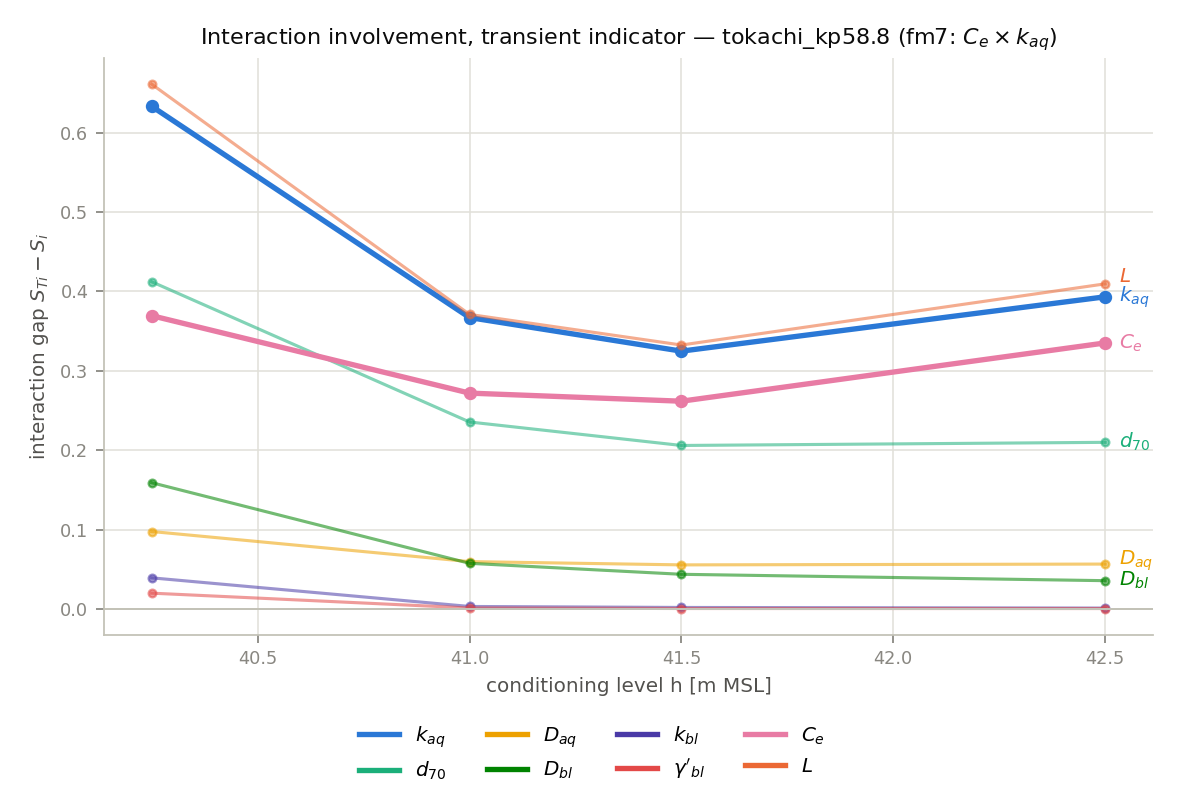
\includegraphics[width=0.72\textwidth]{figures/gsa_interaction_kp58_8_matrix.png}
  \caption[Interaction gap along the conditioning axis, KP58.8]{Interaction
    involvement $S_{Ti} - S_i$ of each input for the transient failure
    indicator along the conditioning axis at KP58.8. The multiplicative
    rate-law pair $C_e$ and $k_{aq}$ (emphasized) retains a large
    interactive share at all levels; toward the fragility shoulder the
    indicator becomes almost purely interactive, which is the mechanism
    behind the vanishing LHS tail advantage found in the convergence
    study.}
  \label{fig:gsa_interaction}
\end{figure}

\paragraph{Level dependence and the +4K reading.}
Figure~\ref{fig:gsa_levels} shows the index rotation along the
conditioning axis for the transient indicator. Rising stages, the
direction in which the +4K hazard shifts probability mass, monotonically
increase the first-order share of $C_e$ (0.011 at the shoulder to 0.114
at the upper level at KP58.8) while the initiation-side inputs $D_{bl}$,
$D_{aq}$, $k_{bl}$, and $\gamma'_{bl}$ fade toward noninfluence; the
composite picture is a shift from an initiation-and-interaction-dominated
regime at survivable stages toward a progression-rate-dominated regime at
extreme stages. Under warming, parameter importance therefore migrates
from the blanket variables toward the erosion-dynamics pair
($C_e$, $k_{aq}$) and the geometry ($L$), which is also the direction in
which the Phase~2 survival evidence is informative.

% --- Figure 3: level dependence ---
\begin{figure}[htbp]
  \centering
  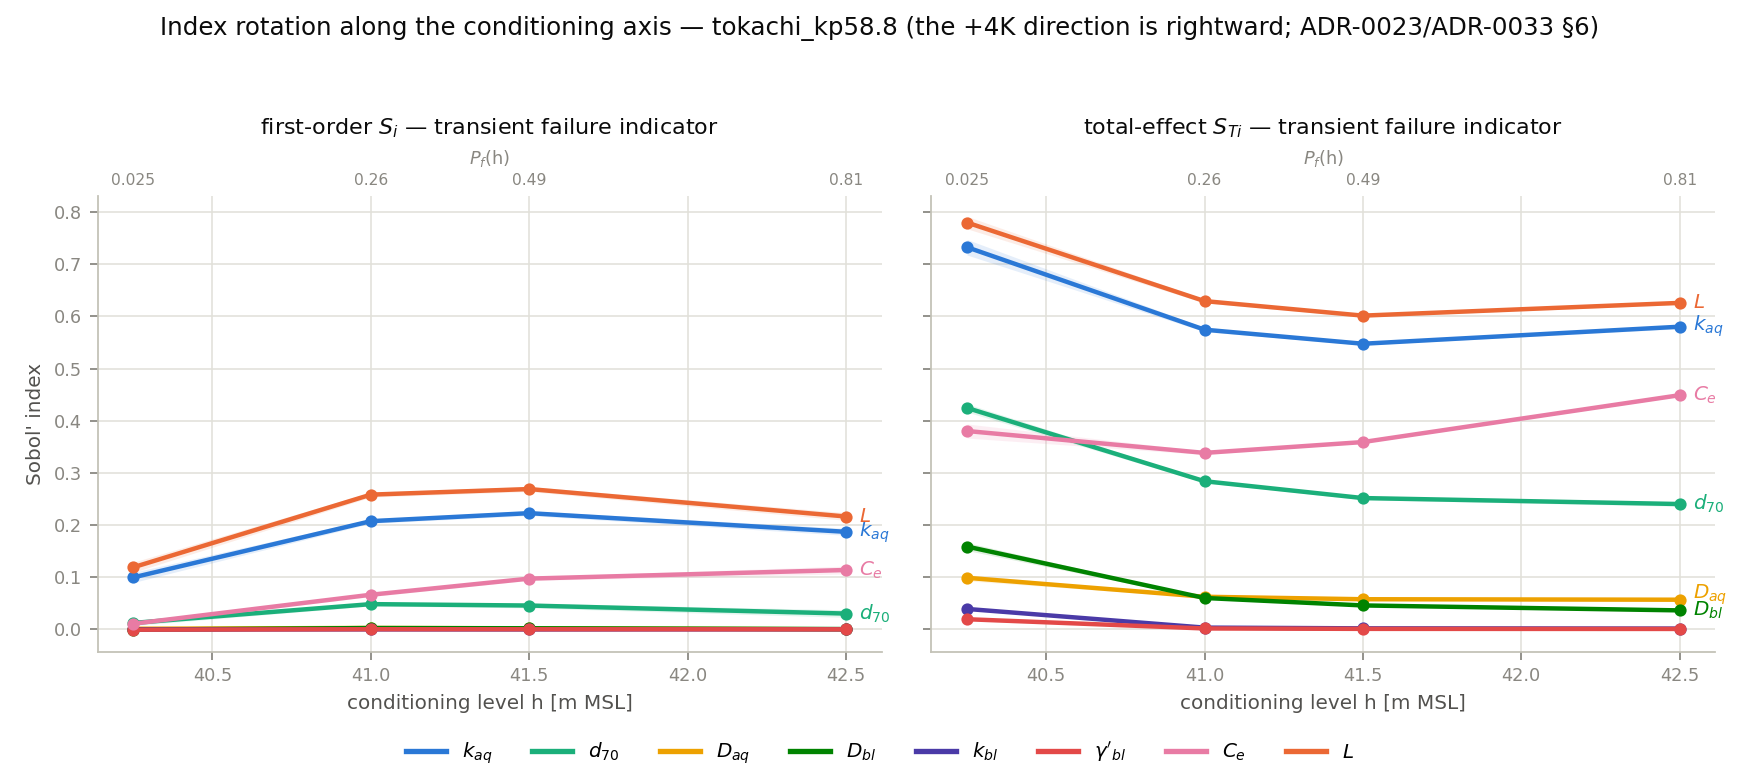
\includegraphics[width=\textwidth]{figures/gsa_levels_kp58_8_matrix.png}
  \caption[Index rotation along the conditioning axis, KP58.8]{First-order
    (left) and total-effect (right) indices of the transient failure
    indicator versus conditioning level at KP58.8, with the per-level
    transient failure probability on the upper axis. The +4K climate
    signal moves probability mass rightward along this axis (ADR-0023),
    so the displayed rotation is the parameter-importance shift under
    warming.}
  \label{fig:gsa_levels}
\end{figure}

\paragraph{Second section.}
KP60.0 reproduces the structure with one leadership swap. At its design
level ($h = 42.75$\,m, transient $P_f = 0.314$) the total-effect ranking is
$k_{aq}$ ($S_T = 0.61$), then $L$ (0.49) and $C_e$ (0.48) statistically
tied, then $d_{70}$ (0.25), with the gate variables again noninfluential
away from the shoulder; first-order shares are $k_{aq}$ 0.25, $L$ 0.16,
$C_e$ 0.15, $d_{70}$ 0.04 ($\sum_i S_i = 0.61$). The static margin
decomposes as $k_{aq}$ 0.43, $L$ 0.30, $d_{70}$ 0.24 with the same exact
structural zeros and level invariance as KP58.8. The membership of the
active set and the interactive character of $C_e$ (first-order 0.15
against total 0.48) therefore replicate across sections, while the
leadership between $k_{aq}$ and $L$ is section-dependent: KP60.0 carries a
lower conductivity population (mean $10^{-3}$\,m/s against
$2 \times 10^{-3}$) and a heavier foreshore damping, which repositions the
population relative to its initiation and progression thresholds. At the
KP60.0 shoulder ($h = 42.0$\,m, $P_f = 0.049$) the interaction dominance
recurs: $\sum_i S_i = 0.32$, with gaps of 0.59 ($k_{aq}$), 0.54 ($L$),
0.48 ($C_e$), and 0.36 ($d_{70}$).

\paragraph{Convergence and uncertainty evidence.}
Across both sections, all reported indices satisfy the pre-registered
criterion (absolute drift below 0.02 between the two finest ladder rungs)
with one class of deliberate exceptions: the static indicator at levels
where its failure probability approaches one (KP58.8 at $h = 42.5$\,m with
$P_f = 0.991$; KP60.0 at $h \geq 43.25$\,m with $P_f \geq 0.98$) sits in
the degenerate-indicator regime where $V(Y) = P_f(1-P_f)$ collapses, is
flagged unconverged in the study records, and is excluded from
interpretation on the same regime grounds as the raw-tail fragility
deliverable (ADR-0024); the level-invariant margin $Y_4$ carries the
static-branch conclusions there. At the operating design ($N = 8192$, $R = 25$), the 95\,\%
replicate intervals on the transient-indicator indices are narrower than
$\pm 0.005$ ($S_i$) and $\pm 0.004$ ($S_{Ti}$) at the KP58.8 design level,
and the pooled bootstrap intervals agree with the replicate intervals to
within about 0.005 in every reported case
(Figure~\ref{fig:gsa_convergence}).

% --- Figure 4: convergence ladder ---
\begin{figure}[htbp]
  \centering
  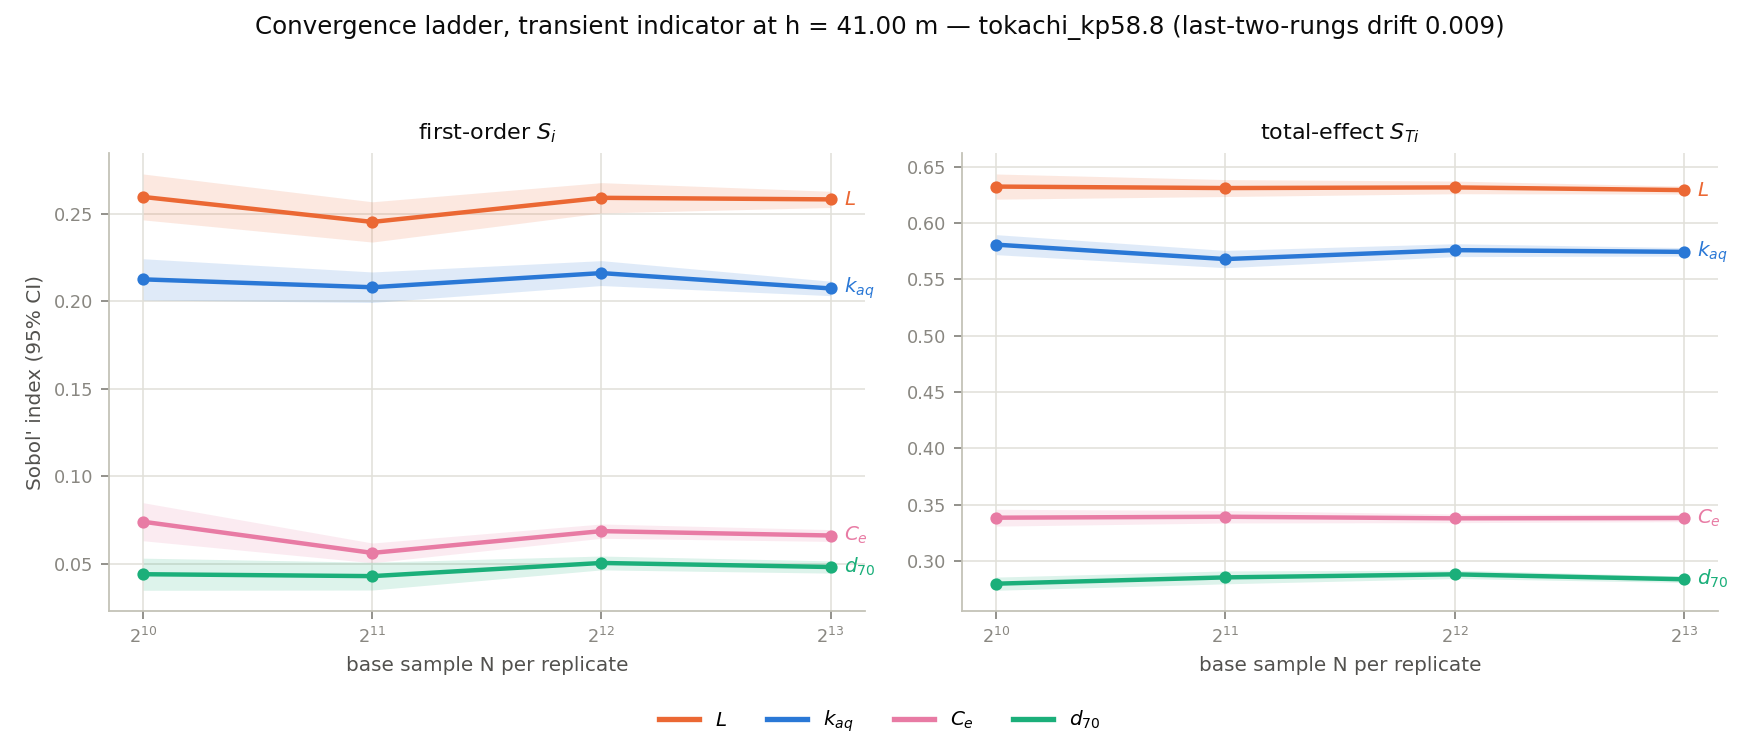
\includegraphics[width=\textwidth]{figures/gsa_convergence_kp58_8_matrix.png}
  \caption[GSA convergence ladder, KP58.8]{Convergence of the four leading
    transient-indicator indices at the KP58.8 design level over the
    $N$-ladder $2^{10}$ to $2^{13}$ (bands: 95\,\% replicate intervals at
    $R = 25$). The estimates stabilize well inside the 0.02 acceptance
    band; the interval width at the final rung is the operating
    uncertainty of the reported indices.}
  \label{fig:gsa_convergence}
\end{figure}

\paragraph{Robustness companions.}
Three companion runs probe the two prior choices most able to move the
ranking (Figure~\ref{fig:gsa_companions}). Under the co-primary
\emph{bulk} $d_{70}$ interpretation (13\,mm framework gravel against the
0.53\,mm matrix sand) the whole KP58.8 fragility shifts about 4\,m upward
and the transient indicator is degenerate at the matrix design stage
($P_f = 0$ at $h = 41.0$\,m), itself a substantive statement about that
interpretation; the comparison is therefore made at the matched curve
position $h = 45.0$\,m ($P_f = 0.154$). There the leading pair is
unchanged ($L$ at $S_T = 0.69$, $k_{aq}$ at 0.62) while the resistance
weight shifts from the erosion dynamics toward the grain size ($d_{70}$
rises to 0.40, $C_e$ falls to 0.16): under a coarse-grain reading,
failures are resistance-selected rather than rate-selected. The two Nataf
companions impose the bounding $\rho_{\ln} = 0.6$ and agree with each
other on the joint distribution as they must (transient $P_f = 0.238$ in
both orderings, against 0.263 independent): the positive correlation
pairs high-conductivity draws with coarse-grain draws whose effects on
the critical head partially cancel, lowering the transient failure
probability and shrinking the soil-resistance share of the variance. The
importance ranking is preserved under dependence ($L$, then $k_{aq}$,
then $C_e$, then $d_{70}$), so no conclusion of this section rests on the
independence adoption of ADR-0012.

% --- Figure 5: companions ---
\begin{figure}[htbp]
  \centering
  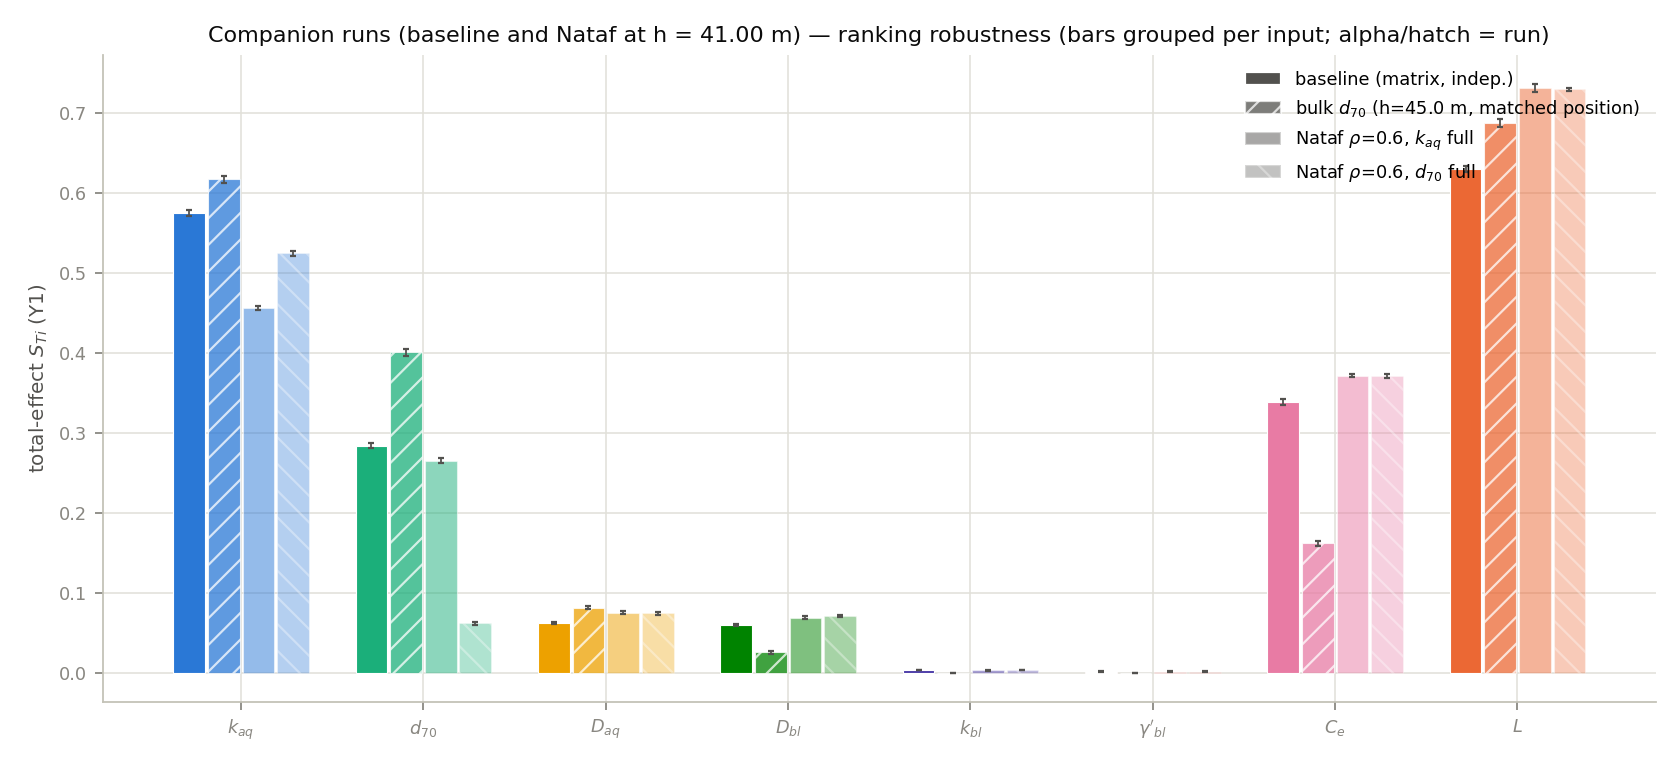
\includegraphics[width=\textwidth]{figures/gsa_companions.png}
  \caption[GSA companion runs at the design level]{Total-effect indices of
    the transient failure indicator at the KP58.8 design level for the
    baseline (matrix $d_{70}$, two-population coupling) against the three
    companions: the bulk $d_{70}$ interpretation and the bounding Nataf
    $\rho_{\ln} = 0.6$ runs in both Rosenblatt orderings (the anchored
    variable carrying the full contribution, the other its independent
    remainder).}
  \label{fig:gsa_companions}
\end{figure}

\subsection{Interpretation and Consequences}
\label{subsec: GSA Interpretation}

\paragraph{Initiation versus progression.}
The GSA separates the two physical stages cleanly. The blanket-side gate
variables ($D_{bl}$, $k_{bl}$, $\gamma'_{bl}$, acting through the
r$_e$-attenuated uplift-heave check) matter only where the fragility curve
has its shoulder, i.e.\ where initiation still discriminates between
realizations; there $D_{bl}$ reaches a total effect of 0.16 at KP58.8.
From the design level upward the transient failure question is decided by
progression dynamics ($C_e$, $k_{aq}$), resistance ($d_{70}$, $D_{aq}$
through the critical head), and geometry ($L$). For prioritizing site
investigation at the survivable stages that dominate the risk integral,
the shoulder picture is the relevant one, and it says: seepage length and
aquifer conductivity first, then grain size and erosion coefficient,
blanket properties last.

\paragraph{The dominant role of the seepage length.}
That $L$, a geometric survey quantity with a modeling-assigned coefficient
of variation of 0.20, out-ranks every soil property at KP58.8 for every QoI
is the single most actionable finding. It implies, first, that the
uncertainty in the Phase~1 fragility curves is to a large extent geometric
rather than geotechnical, and can be reduced by cross-section surveying
and seepage-path interpretation rather than by additional soil testing;
second, that the sensitivity of the deliverable to the assigned
$\mathrm{CoV}(L) = 0.20$ itself warrants care when that value is revisited;
and third, a structural consequence for Phase~2: the Accept-Reject
filtering operates on the seven-column $\theta$ matrix, while $L$ is drawn
independently per cross-section, so survival evidence will tighten the
soil-parameter posterior but leave the dominant geometric uncertainty
untouched. Any future claim that Phase~2 calibration has strongly reduced
fragility uncertainty must be read against this ceiling.

\paragraph{What Phase 2 can and cannot learn.}
$C_e$'s influence on the failure indicator is predominantly interactive
(first-order 0.07 against total 0.34 at the design level). For Bayesian
updating this has a concrete meaning: the 2016 survival observation, which
acts through the transient indicator at the realized stages, carries
limited marginal information on $C_e$ alone but substantial information on
the joint tail of ($C_e$, $k_{aq}$, $L$, $d_{70}$). The posterior should
therefore be expected to contract along the multiplicative
high-rate corner (the failure-mode-7 direction) rather than along the
$C_e$ axis by itself, and marginal posterior standard deviations will
understate what was actually learned. This sharpens the survival
discrimination framing of the architecture specification: the transient
rejection set is an interaction-shaped region, not a box.

\paragraph{Static-transient bias attribution.}
The comparator contrast localizes the bias mechanism. The static and
transient branches share their resistance backbone ($L$, $k_{aq}$,
$d_{70}$, $D_{aq}$ order identically in $Y_2$ and $Y_1$), so the bias
between the curves is carried not by a re-ranking of shared parameters but
by the two transient-only mechanisms: the erosion-dynamics pair
($C_e$ at $S_T = 0.34$) and, at shoulder levels, the initiation gate
($D_{bl}$ at 0.16). This is consistent with the four-component gap
decomposition of the architecture specification: the temporal and
dimensional components act through the parameters both branches share,
while the finite-rate component is exactly the $C_e$ sensitivity the
static branch cannot see.

\paragraph{Correlation robustness.}
The Nataf companion also illustrates, on the production physics, why the
dependent-input decomposition must be handled explicitly rather than by
running independent-input formulas on correlated samples. Under
$\rho_{\ln} = 0.6$ the \emph{full} contribution of $d_{70}$ to the static
margin nearly vanishes ($S = 0.01$, against an independent contribution
of 0.18): the correlated share of $k_{aq}$ moves the critical head in the
opposite direction and almost exactly cancels the grain-size effect. A
full index smaller than the corresponding independent index is a
signature phenomenon of dependent inputs
\parencite{mara_tarantola_2012, kucherenko_2012} and would be
uninterpretable, or worse, silently wrong, under a naive treatment. For
the engine's conclusions the operative statement is negative and
reassuring: even at a correlation six times the empirical estimate, the
transient importance ranking is unchanged and the dominant-input finding
($L$) is strengthened rather than weakened.

\paragraph{Limitations.}
The indices are properties of the model and its prior jointly: they are
conditional on the ADR-0026 $C_e$ field prior (whose coefficient of
variation 0.78 is itself the widest in the vector), on
$\mathrm{CoV}(L) = 0.20$, and on the two-population coupling; a revised
prior re-weights the decomposition. Indicator QoIs lose statistical
meaning where $P_f$ approaches 0 or 1 (the degenerate static level above),
and the shoulder-level indicator indices, while converged under the
criterion, carry the widest intervals of the study. Finally, the analysis
is per cross-section; it inherits the engine's scope (no length-effect
upscaling) and says nothing about segment-scale importance until the
autocorrelation length is fixed.

% =========================================================================
% End of GSA section
% =========================================================================
